\begin{enumerate}
	\item \textbf{Validate User}
		\begin{enumerate}
			\item \textbf{Service Contract}
				\begin{figure}[H]
					\centering
					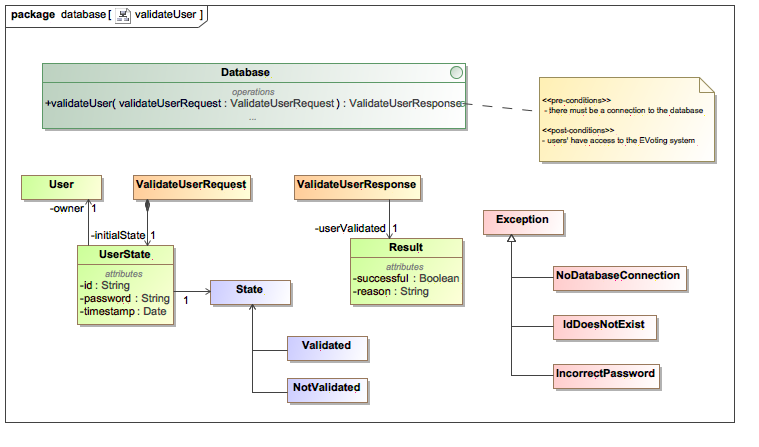
\includegraphics[width=0.75\linewidth]{../Images/Database/ServiceContracts/ValidateUser_ServiceContract.png}
					\caption{Validate User Service Contract}
				\end{figure}
				
				*insert discription here*
				\newline				
				
				\begin{enumerate}
					\item Pre-conditions
					\begin{itemize}
						\item There must be a connection to the database
					\end{itemize}
					
					\item Exceptions
					\begin{itemize}
						\item If there is no connection to the database, the NoDatabaseConnection exception will be thrown
						\item If a user's ID is not valid, the IdDoesNotExist exception will be thrown
						\item If the user's password is entered incorrectly, the IncorrectPassword exception will be thrown
					\end{itemize}
					
					\item Post-conditions
					\begin{itemize}
						\item Users have access to the EVoting system
					\end{itemize}
				\end{enumerate}
			
			\item \textbf{Functional Requirements}
				\begin{figure}[H]
					\centering
					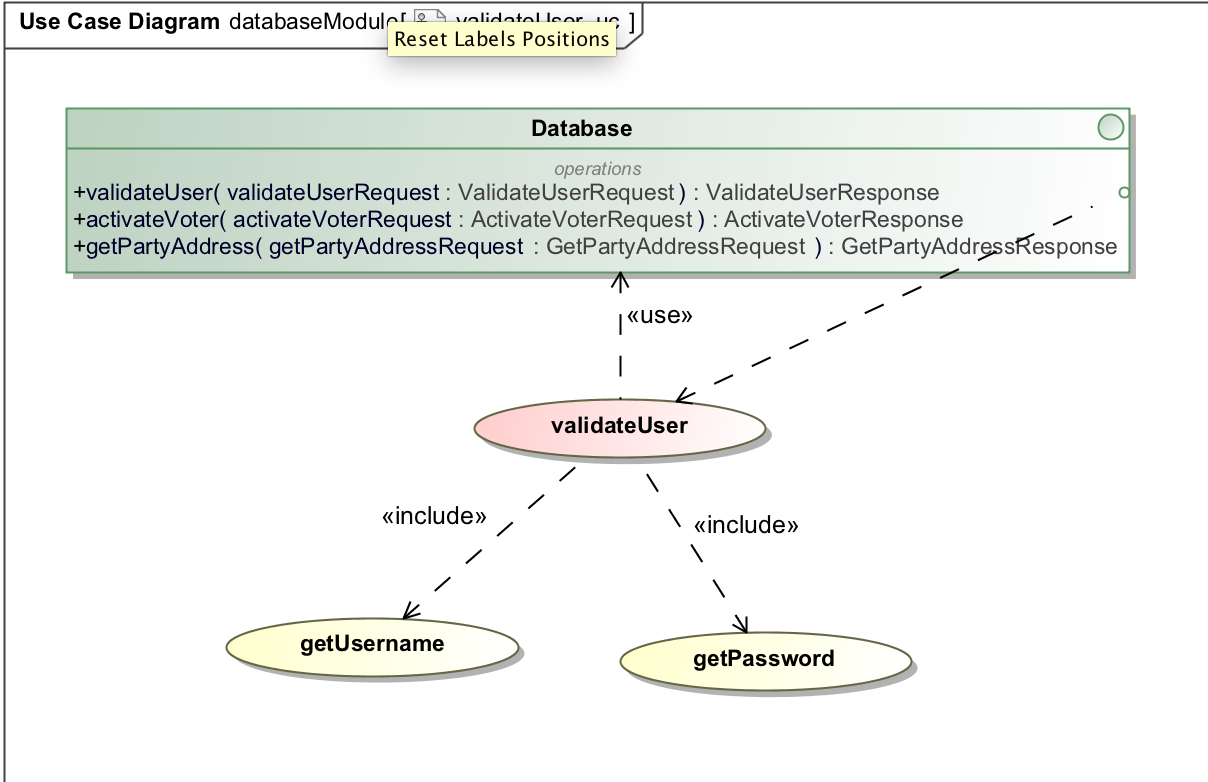
\includegraphics[width=0.75\linewidth]{../Images/Database/UseCases/ValidateUser_UseCase.png}
					\caption{Validate User Use Case}
				\end{figure}
				
				*insert discription here*
				\newline
			
			\item \textbf{Process Design}
				\begin{figure}[H]
					\centering
					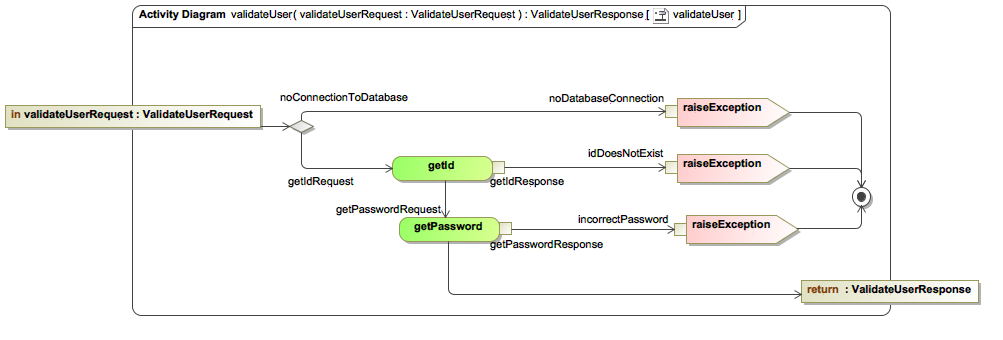
\includegraphics[width=0.75\linewidth]{../Images/Database/Activity/ValidateUser_Activity.png}
					\caption{Validate User Activity}
				\end{figure}
				
				*insert discription here*
				\newline
		\end{enumerate}
	
	\item \textbf{Activate User}
		\begin{enumerate}
			\item \textbf{Service Contract}
			\begin{figure}[H]
				\centering
				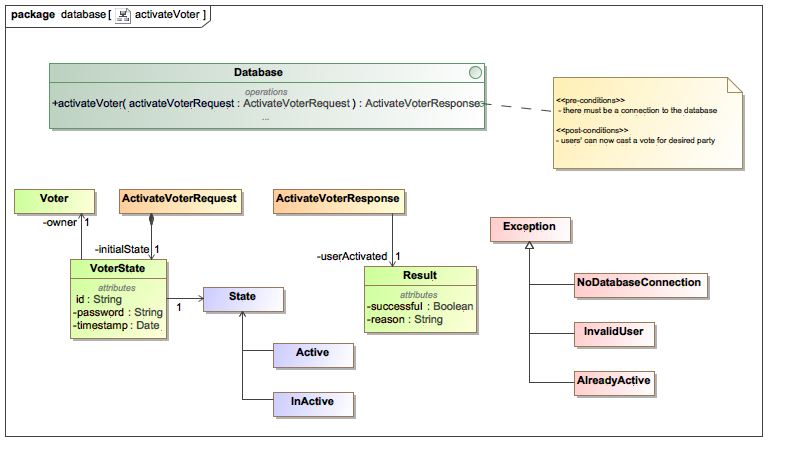
\includegraphics[width=0.75\linewidth]{../Images/Database/ServiceContracts/ActivateVoter_ServiceContract.png}
				\caption{Activate Voter Service Contract}
			\end{figure}
			
			*insert discription here*
			\newline
			
			\begin{enumerate}
				\item Pre-conditions
				\begin{itemize}
					\item There must be a connection to the database
				\end{itemize}
				
				\item Exceptions
				\begin{itemize}
						\item If there is no connection to the database, the NoDatabaseConnection exception will be thrown
						\item If a user could not be validated, the InvalidUser exception will be thrown
						\item If the user has already been activated, the AlreadyActive exception will be thrown
				\end{itemize}
				
				\item Post-conditions
				\begin{itemize}
					\item Users can now cast a vote for their desired party
				\end{itemize}
			\end{enumerate}
			
			\item \textbf{Functional Requirements}
			\begin{figure}[H]
				\centering
				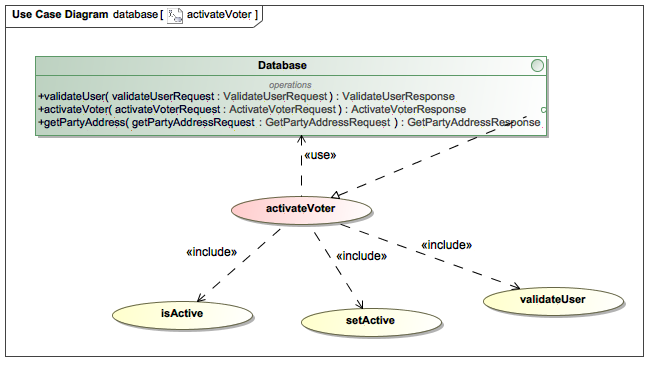
\includegraphics[width=0.75\linewidth]{../Images/Database/UseCases/ActivateVoter_UseCase.png}
				\caption{Activate Voter Use Case}
			\end{figure}
			
			*insert discription here*
			\newline
			
			\item \textbf{Process Design}
			\begin{figure}[H]
				\centering
				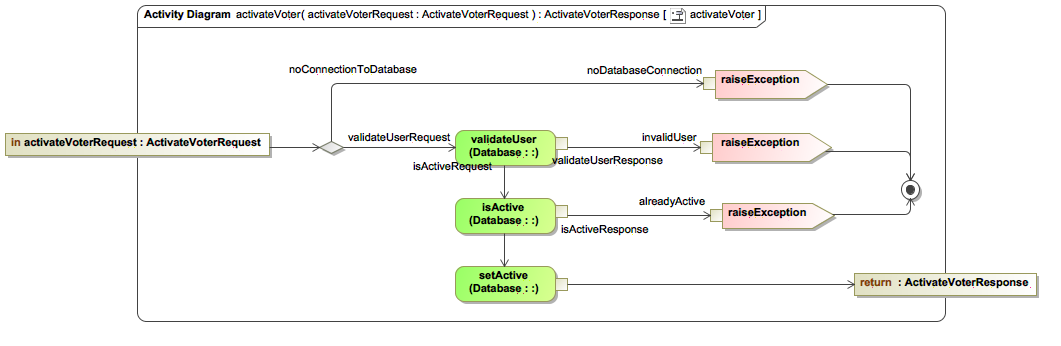
\includegraphics[width=0.75\linewidth]{../Images/Database/Activity/ActivateVoter_Activity.png}
				\caption{Activate Voter Activity}
			\end{figure}
			
			*insert discription here*
			\newline
		\end{enumerate}
\end{enumerate}